
%%% Local Variables:
%%% LaTeX-command: "pdflatex --shell-escape"
%%% End:

\documentclass[11pt]{article}
\usepackage[utf8]{inputenc}
\usepackage[T1]{fontenc}
\usepackage{grffile}
\usepackage{longtable}
\usepackage{wrapfig}
\usepackage{rotating}
\usepackage[normalem]{ulem}
\usepackage{amsmath}
\usepackage{textcomp}
\usepackage{amssymb}
\usepackage{capt-of}
\usepackage{hyperref}
\hypersetup{colorlinks=true, linkcolor=magenta}
\setlength{\parindent}{0in}
\usepackage[margin=0.8in]{geometry}
\usepackage[english]{babel}
\usepackage{mathtools}
\usepackage{palatino}
\usepackage{fancyhdr}
\usepackage{sectsty}
\usepackage{engord}
\usepackage{parskip}
\usepackage{minted}
\usepackage{cite}
\usepackage{graphicx}
\usepackage{subcaption}
\usepackage{setspace}
\usepackage[compact]{titlesec}
\usepackage[center]{caption}
\usepackage{placeins}
\usepackage{color}
\usepackage{amsmath}
\usepackage{bm}
\usepackage{todonotes}
\usepackage{pdfpages}
% \titlespacing*{\subsection}{0pt}{5.5ex}{3.3ex}
% \titlespacing*{\section}{0pt}{5.5ex}{1ex}
\author{Luis Antonio Ortega Andrés\\Antonio Coín Castro}
\date{}
\title{Fingerprint Biometrics Lab - Report\\\medskip
\large APRENDIZAJE PROFUNDO PARA PROCESAMIENTO DE INFORMACIÓN BIOMÉTRICA}
\hypersetup{
 pdfauthor={Luis Antonio Ortega Andrés},
 pdftitle={},
 pdfkeywords={},
 pdfsubject={},
 pdflang={Spanish}}}

\begin{document}

\maketitle

\section*{Exercise 1}
\textbf{a) } \emph{Copy here the two fingerprint images provided as examples (\texttt{example1\_1} and \texttt{example1\_2})}.

\begin{figure}[h!]
  \centering
       \begin{subfigure}[t]{0.45\textwidth}
         \centering
         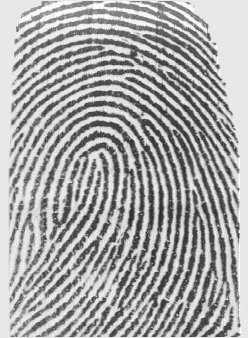
\includegraphics[scale=0.8]{img/example1_1.png}
         \caption{Example1\_1}
     \end{subfigure}%
     \quad
     \begin{subfigure}[t]{0.45\textwidth}
         \centering
         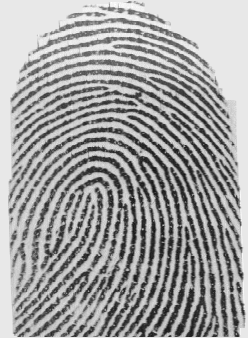
\includegraphics[scale=0.8]{img/example1_2.png}
         \caption{Example1\_2}
     \end{subfigure}
    \caption{Original fingerprints.}
    \label{fig:ex1a}
\end{figure}

\textbf{b) } \emph{How many macro-singularities do you observe in each fingerprint?}

We can see in Figure \ref{fig:ex1a} that there is only one macro-singularity in each fingerprint. Specifically, we observe a \textbf{loop} in each one of them, around the centre of each image. There are no \textit{deltas} or \textit{whorls}.

\textbf{c) } \emph{Mark the macro-singularities in the images (deltas and loops).}

The result of marking each of the loops in shown in Figure \ref{fig:ex1c}. To avoid cluttering the images, we only point out the zones in which the ``U'' shape is most notable.

\begin{figure}[h!]
  \centering
       \begin{subfigure}[t]{0.45\textwidth}
         \centering
         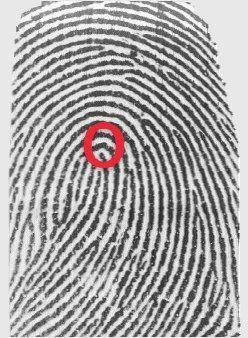
\includegraphics[scale=0.6]{img/msing_1.jpg}
         \caption{Example1\_1}
     \end{subfigure}%
     \quad
     \begin{subfigure}[t]{0.45\textwidth}
         \centering
         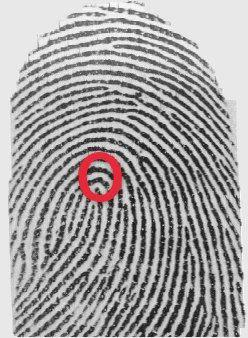
\includegraphics[scale=0.6]{img/msing_2.jpg}
         \caption{Example1\_2}
     \end{subfigure}
    \caption{Macro-singularities (loops).}
    \label{fig:ex1c}
\end{figure}

\newpage
\section*{Exercise 2}

\textbf{a) }\emph{Execute the provided code for Fingerprint Enhancement and paste the resulting image here.}

The resulting image is shown in Figure \ref{fig:ex2a}.

\begin{figure}[h!]
  \centering
       \begin{subfigure}[t]{0.45\textwidth}
         \centering
         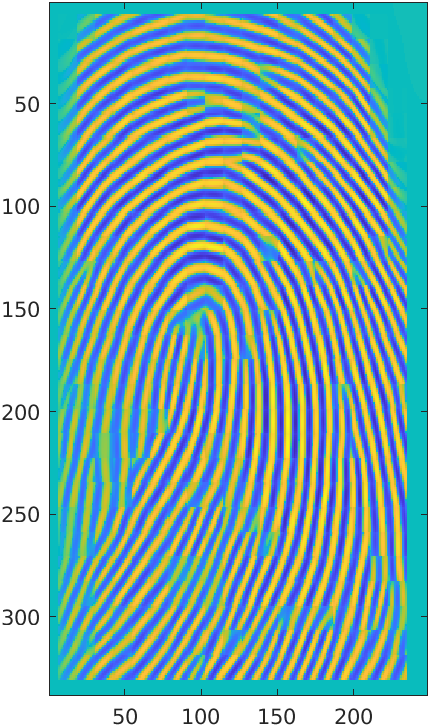
\includegraphics[scale=0.7]{img/enhanced_1}
         \caption{Example1\_1}
     \end{subfigure}%
     \quad
     \begin{subfigure}[t]{0.45\textwidth}
         \centering
         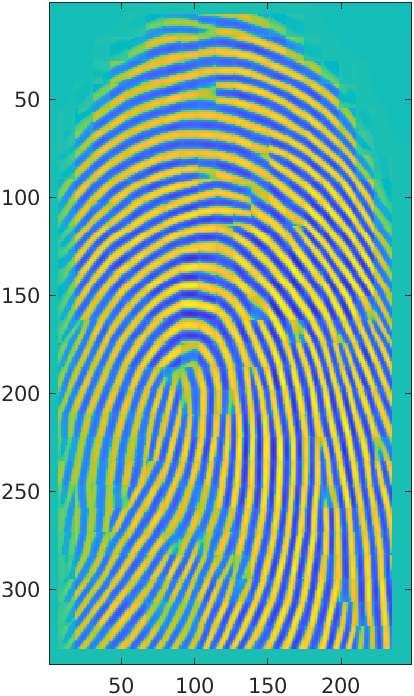
\includegraphics[scale=0.725]{img/enhanced_2}
         \caption{Example1\_2}
     \end{subfigure}
    \caption{Fingerprint Enhancement.}
    \label{fig:ex2a}
\end{figure}


\textbf{b) }\emph{What differences do you observe with respect to the original fingerprints?}

Fingerprint enhancement facilitates the identification of ridge-valley structures and hence the features of each fingerprint. More precisely, we obtain a representation where any intermittent stroke of a ridge is replaced with a continuous one, and also contrast enhancement is performed. As we can see in Figure \ref{fig:ex2a}, the differences with respect to Figure \ref{fig:ex1a} are that the ridge lines are continuous, smoother, and can be distinguished more clearly from the background.\\

\section*{Exercise 3}

\textbf{a) }\emph{Execute now the code for Quality Maps, and paste the resulting quality maps.}

The resulting quality maps are shown in Figure \ref{fig:ex3a}.

\begin{figure}[h!]
  \centering
       \begin{subfigure}[t]{0.45\textwidth}
         \centering
         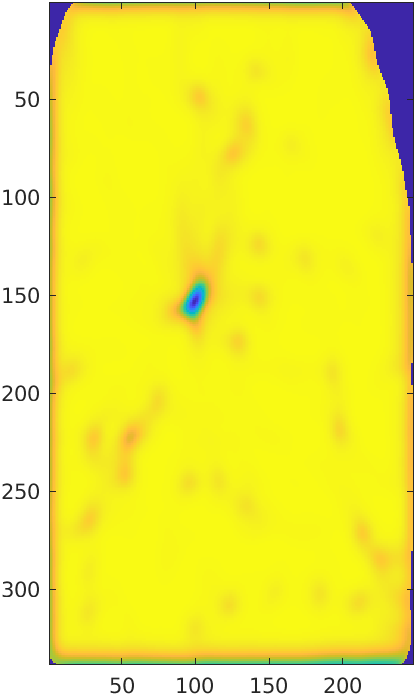
\includegraphics[scale=0.7]{img/qmap_1}
         \caption{Example1\_1}
     \end{subfigure}%
     \quad
     \begin{subfigure}[t]{0.45\textwidth}
         \centering
         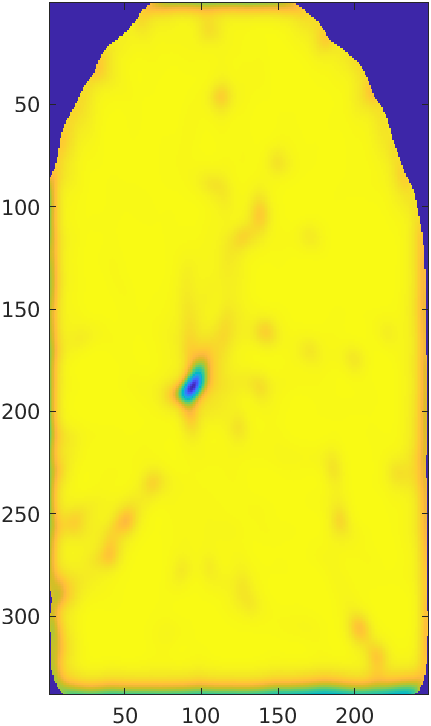
\includegraphics[scale=0.675]{img/qmap_2}
         \caption{Example1\_2}
     \end{subfigure}
    \caption{Fingerprint Quality Maps.}
    \label{fig:ex3a}
\end{figure}

\textbf{b) }\emph{What is the range of values for these quality maps?}

Inspecting each matrix by hand, we can see that for both images the minimum value (shown in dark blue) is \( 0.0 \), while the maximum values (shown in yellow) are \( 0.9991 \) and \(  0.9988 \) for \verb@Example1_1@ and \verb@Example1_2@, respectively. Given this, we can assume that the range of values for the quality is \( [0, 1] \).

\textbf{c) }\emph{What kind information (apart from the quality) can be inferred from such code?}

Inspecting the given source code, we conclude that the heat map displayed in Figure \ref{fig:ex3a}} corresponds to a measure of the reliability of the computed orientation for each ridge (by means of the function \verb@ridgeorient@). We can think of this quantity as a measure of the reliability of the computed enhancement for each fingerprint, that is, how well the computed orientation resembles the real outline of the ridge curves.

Taking a look into our examples, there is one region where the reliability is low (blue), which corresponds to the sharpest point of the loop. This results is intuitive given that those points are the ones where the orientation changes abruptly, leading to less accurate results.


\section{Exercise 4}

\emph{Execute the code in order to show the Binarized Fingerprint and the Segmented Fingerprint. Apply different values of quality threshold (0.1, 0.3, 0.6, 0.9) and paste here the resulting images:}

\begin{figure}
  \centering
  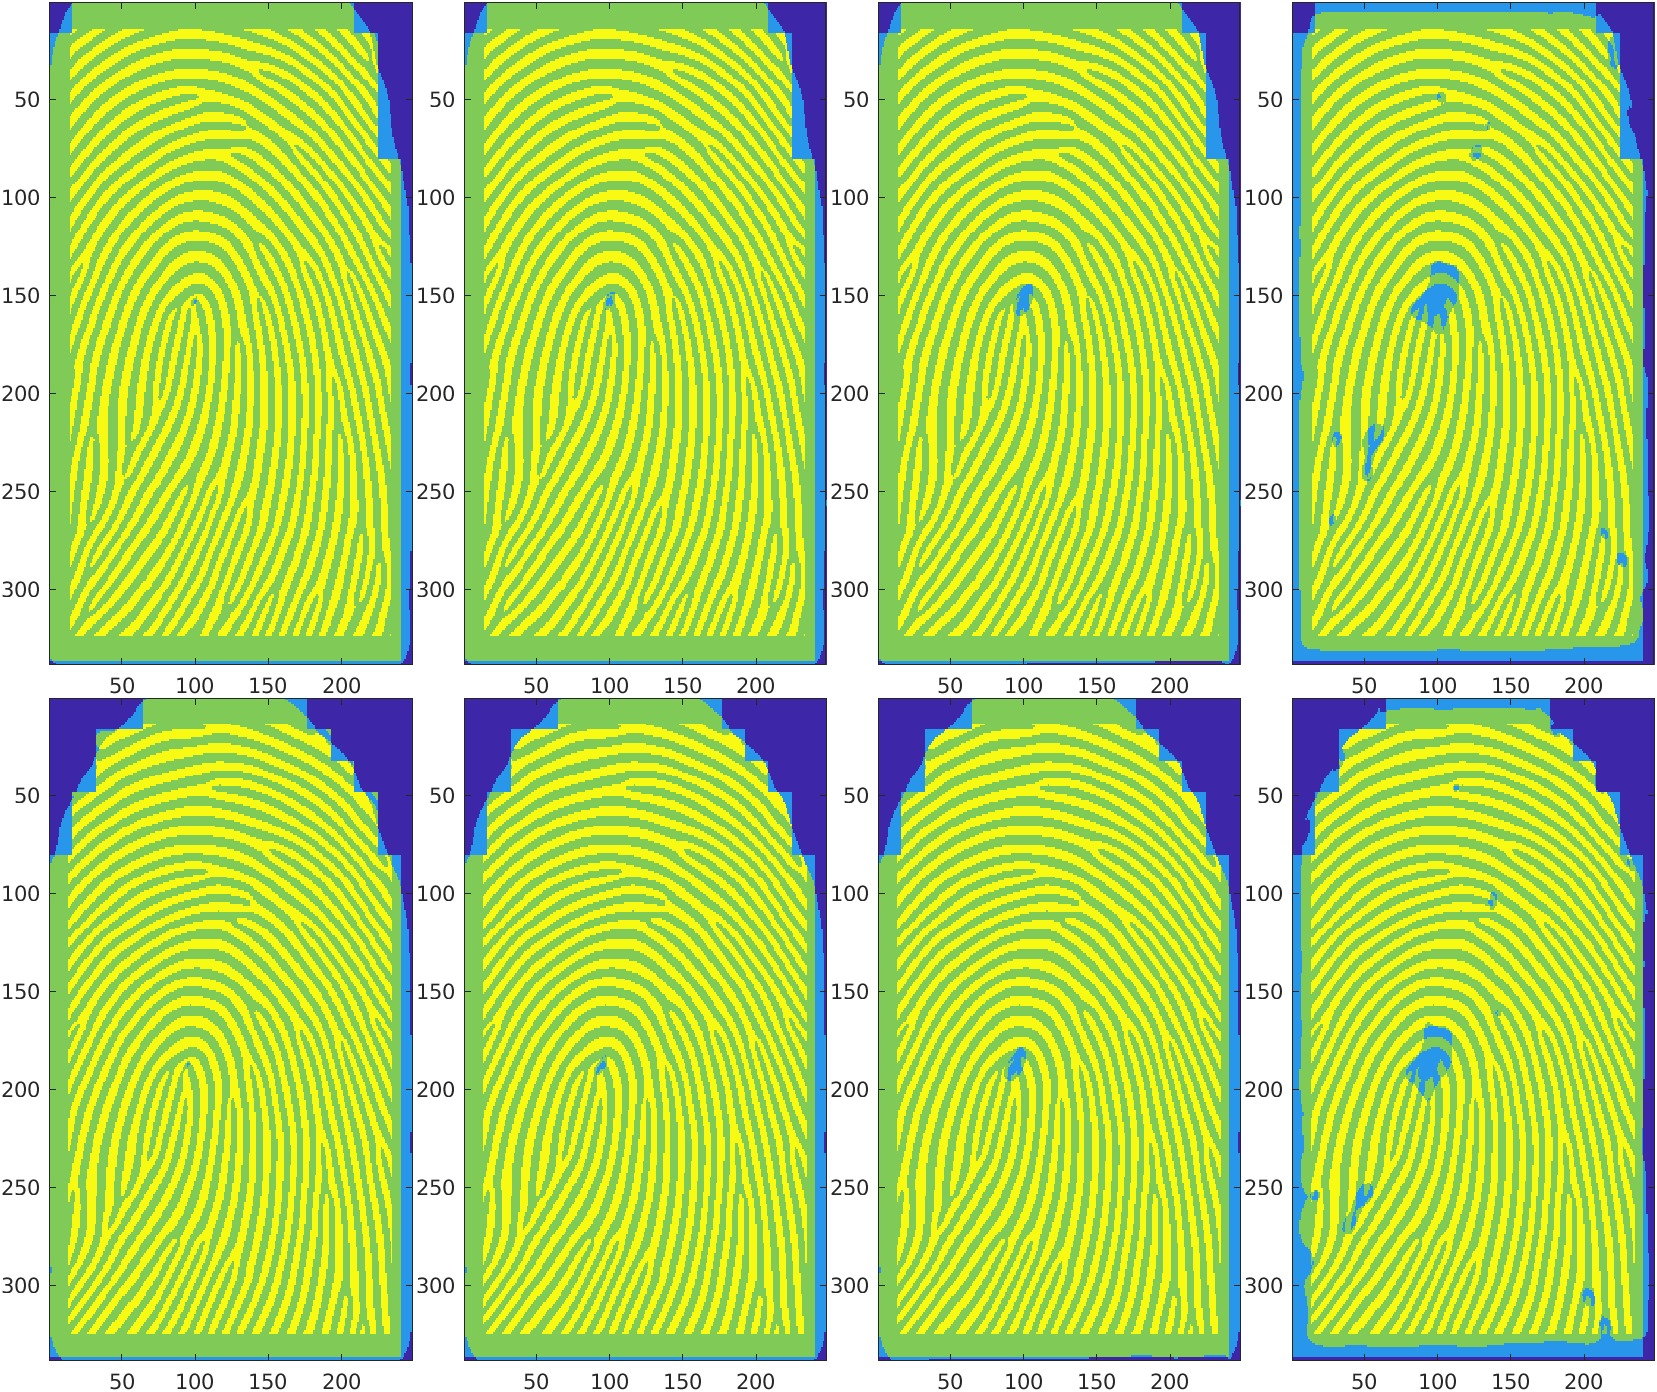
\includegraphics[scale=0.5]{img/merge_bin}
  \caption{Example1\_1 and Example1\_2 (first and second row) Binarized and Segmented Fingerprint with thresholds 0.1, 0.3, 0.6 and 0.9 (columns).}
\end{figure}

\section{Exercise 5}

\textbf{a) }\emph{Execute the code for generating the Fingerprint Skeleton and the Minutiae Extractor. Paste the resulting images for the original values window=5 and margin=5.}

\textbf{b) }\emph{Search heuristically by looking at the images for the optimal values of parameters window and margin. Paste the resulting images with your optimal parameters and justify your decision.}

\section{Exercise 6}

\textbf{a) }\emph{Execute the code corresponding to the Minutiae Validation for window=5 and margin=5.  Paste the resulting image including the minutiae extracted (red crosses) and validated (blue circles) of both fingerprints. }

\textbf{b) }\emph{Execute the same code but with the optimal values of parameters window and margin. Paste the resulting image below.}

\textbf{c) }\emph{Do you think it is a good idea to include the Minutiae Validation module? Justify your opinion.}

\section{Extra Exercise}

\emph{In folder \texttt{/ddbb} you have 20 fingerprint images. 19 of them are labeled with the subject identity (e.g., H0001), and 1 is Unknown. Search for the identity of the Unknown fingerprint in the set of 19 labelled reference fingerprints. You can use the provided code \texttt{identification\_1\_19.m} as basis. Paste here the resulting ranked list of scores of the Unknown fingerprint with respect each one of the 19 reference fingerprints.}

- Extrac_window=3, extract_margin=11; val_window=1:
Vector de scores:
`0.186047 0.152542 0.204545 0.153846 0.122066 0.13617 0.173913 0.231884 0.175824 0.176471 0.133333 0.2 0.55 0.197802 0.15873 0.197531 0.204082 0.126984 0.202247`

---> Extrac_window=3, extract_margin=11; val_window=3 (LA QUE MEJOR VA):
Vector de scores:
`0.259887 0.229508 0.26455 0.215385 0.196474 0.195122 0.223776 0.261438 0.224138 0.20339 0.20442 0.235294 0.654206 0.23622 0.203947 0.228916 0.231156 0.2 0.239316`

- Extrac_window=5, extract_margin=5; val_window=1 (POR DEFECTO DEL PROFESOR):
Vector de scores:
`0.205128 0.157895 0.183908 0.15625 0.115385 0.123348 0.170543 0.215385 0.157303 0.168421 0.12844 0.179487 0.526316 0.2 0.156522 0.179487 0.189474 0.122222 0.183908`

- Extrac_window=3, extract_margin=7; val_window=3
Vector de scores:
`0.323741 0.261628 0.285714 0.281609 0.263692 0.280079 0.287263 0.297872 0.306189 0.251572 0.273543 0.285714 0.766667 0.337748 0.282723 0.268551 0.287671 0.264901 0.278912`

EXTRACT_WINDOW: Si aumenta, aumenta la ventana de referencia.
EXTRACT_MARGIN: Elimina los puntos en los bordes, cuanto mayor sea. Hemos encontrado que si es <10 encuentra muchos puntos en los bordes.
VALIDATION_WINDOW: Ventana a partir de la cual borrar puntos. Cuanto mayor es, más puntos borra.


Conclusiones:

- Con más puntos aumenta el score de la 13, pero también aumenta el del resto.
\end{document}
